\documentclass[10pt, openany]{book}

\usepackage[sc]{mathpazo}
\linespread{1.03}
\usepackage[a4paper,width=150mm,top=25mm,bottom=25mm]{geometry}
\usepackage{booktabs}
\usepackage{float}
\usepackage{array}
\usepackage[T1]{fontenc}
\usepackage[utf8]{inputenc}
\usepackage{microtype}
\usepackage[english]{babel}
\usepackage{hyperref}
\usepackage[usenames,dvipsnames]{xcolor}
\usepackage[hang,small,labelfont=bf,up,textfont=it,up]{caption}
\usepackage[normalem]{ulem}
\usepackage{setspace}
\usepackage{fancyhdr}
\usepackage{soul}
\usepackage{graphicx}
\usepackage{pdfpages}
\usepackage{parskip}
\usepackage{tikz}
\usepackage[toc]{glossaries}
\usetikzlibrary{positioning,arrows}

\pagestyle{fancy}
\fancyhf{}
\fancyhead[L]{Design and Implementation of an Adv. Rendered Screensaver}
\fancyhead[R]{By James Balajan}
\fancyfoot[C]{\thepage}
\renewcommand{\headrulewidth}{1pt}
\renewcommand{\footrulewidth}{1pt}
\fancypagestyle{plain}{
\pagestyle{fancy}}

\graphicspath{ {images/} }

\urlstyle{rm}


\makeglossaries

\newglossaryentry{atmospheric-scattering}
{
	name={Atmospheric Scattering},
	text={atmospheric scattering},
	description={Atmospheric scattering, in the context of computer graphics, refers to the modeling and emulation of the process by which light particles are scattered by particles in the atmosphere. Scattering from these particles leads to the blue color of our sky at noon, and its orange color at dawn and dusk}
}

\newglossaryentry{pbr}
{
	name={Physically Based Rendering},
	text={physically based rendering},
	description={In its broadest sense, physically based rendering refers to the usage of physics equations to accurately emulate the trajectories of photons when in contact with materials. An example of a physically based lighting model is the Cook-Torrance model, as opposed to the old, non-physically based Blinn-Phong model}
}

\newglossaryentry{volumetric-clouds}
{
	name={Volumetric Clouds},
	text={volumetric clouds},
	description={Volumetric clouds are rendered using the technique of \gls{volumetric-raymarching} over real-time generated volumes that are designed to emulate the shapes and behaviours of clouds}
}

\newglossaryentry{volumetric-raymarching}
{
	name={Volumetric Raymarching},
	text={volumetric raymarching},
	description={Volumetric raymarching is a graphics technique used to accurately render \gls{participating-media}, such as smoke, fog and clouds}
}

\newglossaryentry{participating-media}
{
	name={Participating Media},
	text={participating media},
	description={Participating media are materials which may absorb, emit and/or scatter light. Participating media usually consist of many particles suspended in the air}
}

\newglossaryentry{shader}
{
	name={Shader},
	text={shader},
	description={a type of computer program originally run on graphics card to do shading, aka lighting simulation. However, shaders now perform a variety of tasks, and the term now refers to a category of computer programs that are designed to be interpreted and run by the graphics card}
}

\newglossaryentry{OpenGL}
{
	name={OpenGL},
	description={a cross-language, cross-platform API standard for rendering 2D and 3D vector graphics. The API is used to interact with a graphics processing unit, to achieve hardware-accelerated rendering}
}

\begin{document}

\pagenumbering{gobble}
\thispagestyle{empty}
\includepdf{external-pdfs/titlepage.pdf}
\pagenumbering{roman}

\tableofcontents
\newpage

\listoffigures
\newpage

\pagenumbering{arabic}

\chapter{Project Proposal}

\begin{figure}[H]
        \centering
        \includegraphics[width=0.35\linewidth]{rainforest}
        \caption{Inspiration for Screensaver. Computer generated Rainforest by Inigo Quilez}
\end{figure} 

\section{Executive Summary}
Much promise has been shown in the applicability of basic, computer generated graphics for creating screen savers for computers in the past, an example of this being that all of the screensavers for Windows XP were rendered. The ability to create aesthetically pleasing, dynamic graphics has made computer generated graphics find use in this field. For this reason a study will be undertaken to investigate if utilising advanced computer graphics techniques to generate a visually appealing scene, which will act as a screensaver, is possible without being overly burdensome on the computer's hardware. Some proposed techniques to be utilised to make this scene are \gls{pbr}, \gls{atmospheric-scattering} and \gls{volumetric-raymarching}, though this list of techniques is subject to change throughout the project as the needs and challenges of the project cannot fully be anticipated.

\begin{figure}[H]
        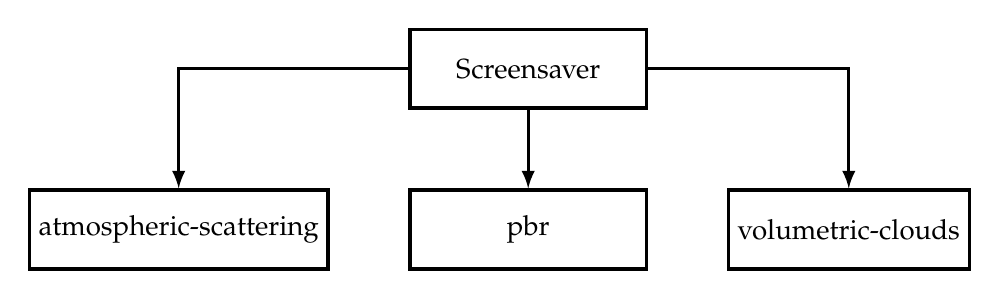
\begin{tikzpicture}
            [%%%%%%%%%%%%%%%%%%%%%%%%%%%%%%
                node distance=1cm,
                box1/.style={rectangle,draw,fill=white!10, very thick,
                              minimum width=3cm, minimum height=1cm},
                box2/.style={align=left,rectangle,draw,fill=gray!10, very thick,
                              minimum width=3cm, minimum height=4cm},
                line/.style={-latex,very thick}
            ]%%%%%%%%%%%%%%%%%%%%%%%%%%%%%%

        \node[box1]             (A) {Screensaver};
	\node[box1, below=of A] (B) {\Gls{pbr}};
	\node[box1, left=of B ] (C) {\Gls{atmospheric-scattering}};
	\node[box1, right=of B] (D) {\Gls{volumetric-clouds}};

        \draw[line] (A.west)  -| (C.north);
        \draw[line] (A.south) -| (B.north);
        \draw[line] (A.east)  -| (D.north);

        \end{tikzpicture}
\caption{Graphics techniques that may be used}
\end{figure} 

To manage the project, the structured approach will be utilised and documented in a portfolio. Our clientele would like for us to use VB.NET to create the project, so the project will be programmed utilising it. As a result, challenges may be faced regarding the performance of the screensaver. Since the development of this screensaver will be only undertaken by one developer, the anticipated completion date of the project is June 2019, although this deadline is subject to change based on circumstances regarding the project.

\chapter{Project Plan}
\section{Defining and Understanding the Problem}
Our initial thoughts on what software construction methodology to use leaned towards one which would benefit a small development team, such as the prototyping methodology. However, it is mandated by our project sponsor that a portfolio be developed to document our development process in a structured manner, so a structured approach is the best choice due to its reliance on documentation.

Thus, the project will be split into 5 stages according to the structured approach:
\begin{itemize}
	\item Planning
	\item Design
	\item Building / Implementing
	\item Testing
	\item Deployment	
\end{itemize}	

These stages are reflected in our Gantt Chart.
Please see figure \ref{fig:gantt} on page \pageref{fig:gantt} for the Gantt Chart.

During the design phase, a survey will be conducted, asking customers what features they would like in a screensaver suite. The survey responses will be considered in our designs and implementation.
After initial implementation, a survey will be conducted requesting the opinions of our customers on the product. As of such, there will be some elements of the prototyping methodology in our approach as well, iterating over our initial product to improve it and satisfy the expectations of our customers. However, as stated previously, the methodology of development will be primarily structured.

\section{Design}
When developing the designs for the product, the following will be created.
\begin{itemize}
	\item A Context Diagram
	\item A Data Flow Diagram	
	\item A Structure Diagram
	\item High level flowcharts for key functions in the program.
	\item A Data Dictionary.
\end{itemize}	
All besides the data dictionary will be created before the implementation stage. The data dictionary will be created along with the product itself.  

\section{Implementation}
The implementation stage will firstly begin with a technical research stage. Advanced graphics techniques involve use of heavy amounts of mathematics, and as of such, research papers must be studied and cited.

After the initial research, implementation will commence. Testing will be done regularly as the project progresses, to ensure each module is functioning before moving onto the next one and to avoid the accumulation of errors. 

\section{Testing}
On completing the implementation, the screensaver suite will be tested on a variety of hardwares, to ensure it functions correctly on other GPUs. This is critical, as graphics \gls{shader}s may perform differently and possibly unexpectedly based on each graphics card provider's \gls{OpenGL} implementation.

\begin{figure}[H]
	\centering
	\includegraphics[width=0.6\linewidth]{project-plan}
	\caption{High-level diagram summarising project plan}
\end{figure}	

\chapter{Feasibility Study}

\section{Executive Summary}

Screensavers have been a medium of graphics experimentation during the times of early computing. However, advanced graphics techniques have never been applied to the context of screensavers, leaving an excellent vacant marketplace to test cutting edge techniques in the context of screensavers. This document analyzes the feasibility of undertaking a project where advanced graphics techniques are applied to create a screensaver from the lenses of technological feasibility, staffing feasibility and marketplace feasibility.

\section{Description of Products and Services}

Screensavers, during the times of early computing, have been the medium for the showcasing of various graphics techniques. From the Windows 98 era with the notable screensaver maze, bringing rasteurized graphics to the customer in a display of engineering creativity to the classic Windows XP pipes, using random generation to provide the customer with a new and consistently unique scene, graphics techniques have found their place in the world of screensavers. However, these screensavers have often been quite basic, using simple Phong shading or even no shading at all with only rasteur based techniques lacking lighting shading. This makes one wonder why advanced graphics techniques, such as the ones explored by video game companies and animation studies such as Pixar, have not been explored in the avenue of screensaver creation. 

\begin{figure}[H]
\centering
\begin{minipage}{.5\textwidth}
  \centering
  \includegraphics[width=.8\linewidth]{maze}
  \captionof{figure}{Windows 98 Maze}
\end{minipage}%
\begin{minipage}{.5\textwidth}
  \centering
  \includegraphics[width=.8\linewidth]{pipes}
  \captionof{figure}{Windows XP Pipes}
\end{minipage}
\end{figure}	

This project aims to investigate this avenue, with the aim of creating a suite of 3 screensavers. The first one will investigate the application of volumetric clouds and randomly generated terrain to screensavers. The second will investigate how mathematical fractal geometry may be applied to generating interesting screensavers. The final will investigate the application of the interesting effect of metaballs to screensavers. 

\begin{figure}[H]
\centering
\begin{minipage}{.3\textwidth}
  \centering
  \includegraphics[width=.9\linewidth]{rainforest}
\end{minipage}%
\begin{minipage}{.3\textwidth}
  \centering
  \includegraphics[width=.9\linewidth]{mandelbrot}
\end{minipage}%
\begin{minipage}{.3\textwidth}
  \centering
  \includegraphics[width=.9\linewidth]{metaballs}
\end{minipage}
\caption{From left to right example images of: Terrain with Volumetric Clouds, Mandelbrot Fractal and Metaballs.}
\end{figure}	

\section{Technology Considerations}

\subsection{Hardware Considerations}

The personnel possess a single HP Pavilion laptop running Windows 10 OS that uses a Nvidia Geforce GTX 1050 graphics card. Although the graphics card is powerful, it is not out of reach of most customers, making it an excellent benchmark for what our users may use.

\subsection{Software Considerations}

The development will be carried out using the VB.NET programming language through the Visual Studio IDE. VB.NET was chosen as a matter of preference from our project sponsor. Due to this unorthodox choice for a programming language for graphics programming, in which C and C++ are most commonly used due to their performance, extra considerations may need to be taken regarding the overhead of the VB.NET language. Furthermore, as VB.NET is being used to create the screensaver suite, the project will only work on the Windows operating system as it requires the .NET framework. However, projects such as .NET core and Mono aim to port the .NET framework to Linux and Mac OSX, so cross compatibility is not completely out of the question, and can be implemented later if the demand is ever shown. 

\section{Product/Service Marketplace}

The marketplace for the utilisation of advanced graphics techniques in the context of screensavers has been fairly limited. No repositories on github were found for screensavers which utilised volumetric clouds, which is not surprising as it is a relatively new graphics technique which is still being researched. No procedural terrain screensavers were found either. This makes the first screensaver idea, of procedurally generated terrain with volumetric clouds, a venture into entirely uncharted territory, as the marketplace is entirely empty.

As for the mandelbrot fractal screensaver, mandelbrot fractals are well documented mathematical structures which produce beautiful results when rendered, however have also, surprisingly not been applied in the context of screensavers. There have, however, been large numbers of mandelbrot fractal explorers generated, as it is seen as an excellent exercise to develop one’s programming skills. An example written in Javascript is shown below:

\begin{figure}[H]
	\centering
	\includegraphics[width=.3\linewidth]{rafrex}
	\caption[Mandelbrot Fractal Rendered by Rafrex's "Fractal"]{Mandelbrot Fractal Renderered by Rafrex's "Fractal" from \url{https://github.com/rafrex/fractal}}
\end{figure}	

Metaballs are also a well documented technique, created by Jim Blinn, the father of Blinn-Phong shading, which produce organic looking balls that change shape depending on their positions relative to other metaballs. Metaballs have been applied to a wide range of areas, however, one particular use of them is in simulating the behaviour of water droplets efficiently, without the use of complex and expensive fluid dynamics simulations. Metaballs have not been applied to the context of screensavers, however, various eye candy demos have been created such as the one below written in Javascript:

\begin{figure}[H]
	\centering
	\includegraphics[width=.3\linewidth]{dynaballs}
	\caption[Metaballs Rendered by FlannelHead's "Dynaballs"]{Metaballs Rendered by FlannelHead's "Dynaballs" from \url{http://flannelhead.github.io/dynaballs/}}
\end{figure}	

\section{Social and Ethical Considerations}

\subsection{Legal Considerations}
As this project is primarily a non-profit, research experiment, the project will be released using the Open Source MIT License. This license limits our liability and makes warranty not legally enforcable, legally protecting us in the case of a potential misuse of our software. The license permits commerical use, modification, distribution and private use of our not for profit, research project.

\subsection{Ergonomics}
\begin{itemize}
	\item The screensaver should be designed to be ergonomic and user friendly. This is easily achievable, as screensavers lack the traditional GUIs of many other products, their main purpose being to be eye candy. Options for these screensavers may be programmed to be directly accessible through the Windows control panel, or could be programmed to be configurable through a separate GUI all together.
	\item The design of the screensaver options dialog will aim to keep the interface simple and intuitive to use, not overflowing the user with unnecessary options. Advanced options will be hidden behind a drop down menu, for experienced users to utilise.
	\item The screensavers will aim to maximise FPS without jeopardising the quality of the screensavers.	
\end{itemize}	

\subsection{Inclusivity}
\begin{itemize}
	\item An English locale will be implemented into the screensaver
suite options dialog, as English is one of the most widely spoken languages in the world. Furthermore, a Russian locale will be implemented as it is the 7th most widely spoken language in the world, and the developer has knowledge of the language. As this project is open source, if more locales are desired to be programmed in, open source contributors may add them.
	\item Data formats that differ internationally, such as dates and currency, are not being handled and hence these factors do not need to be accounted for.
	\item The screensaver would be free and released under the open source licence, allowing anyone of any economic background to utilise it.
	\item The scenes rendered in the screensavers will be designed to be universally appealing to all demographics.	
	\item The option for the screensaver to play music may be programmed in at a later date. One option used to cater for people with hearing disabilities in software is to include subtitles. However, this solution is not suitable, as the person would still not be able to experience the music through a simple text prompt which says "Music Plays". As of such, this issue will be left open to the open source community to solve, if a solution is found in the future.
	\item People with visual impairments must also be catered for. Legal blindness cannot be catered for, as the product is a purely visual one. However, for people with mild visual impairments, text can be written using a clear serif or sans-serif font with a large font size. Poor color combinations will be avoided like yellow on white, only using colors which contrast well, such as black on white.
	\item Issues pertaining to cultural inclusivity need not be worried about, as the screensavers aim to have universal beauty, showcasing the remarkable natures of both the natural and mathematical worlds. 	
\end{itemize}	

\section{Organization and Staffing}

In considering to create this product, considerations must be made regarding whether the developers of this project possess the expertise and the technology required to complete the project. The development team consists of one student programmer, indicating that the personnel may lack the expertise required to develop an advanced graphics screensaver. However, the deadline for the end of the project provides enough time for the programmer to research and become knowledgable on these techniques before implementation.

\section{Schedule}

The schedule of this project will closely follow the Gantt Chart.
The structure of this gantt chart aims to reflect the standard software development life cycle.

\begin{figure}[H]
	\centering
	\makebox[\textwidth][c]{\includegraphics[width=1.2\linewidth]{gantt}}%
	\caption{Gantt chart}
	\label{fig:gantt}
\end{figure}	

\section{Financial Projections}

As the project manager is also the developer and has direct interests in completing this project, the developer demands no pay.
No extra software must be purchased, as all tools that will be used are free.
The only costs associated with this project are those associated with electricity for recharging the laptop.

\section{Findings and Recommendations}

In summary:
\begin{itemize}
	\item There is ample time for research, development and refinement.
	\item Through investigating advanced graphics techniques in screensavers, one can set the groundwork for their future integration into other mediums such as animated movies and video games.
	\item The cost of development is negligible.	
\end{itemize}	
Hence, it is in our best interests that the project proceed.

\printglossaries

\end{document}
